\documentclass{article}\usepackage[]{graphicx}\usepackage[]{color}
%% maxwidth is the original width if it is less than linewidth
%% otherwise use linewidth (to make sure the graphics do not exceed the margin)
\makeatletter
\def\maxwidth{ %
  \ifdim\Gin@nat@width>\linewidth
    \linewidth
  \else
    \Gin@nat@width
  \fi
}
\makeatother

\definecolor{fgcolor}{rgb}{0.345, 0.345, 0.345}
\newcommand{\hlnum}[1]{\textcolor[rgb]{0.686,0.059,0.569}{#1}}%
\newcommand{\hlstr}[1]{\textcolor[rgb]{0.192,0.494,0.8}{#1}}%
\newcommand{\hlcom}[1]{\textcolor[rgb]{0.678,0.584,0.686}{\textit{#1}}}%
\newcommand{\hlopt}[1]{\textcolor[rgb]{0,0,0}{#1}}%
\newcommand{\hlstd}[1]{\textcolor[rgb]{0.345,0.345,0.345}{#1}}%
\newcommand{\hlkwa}[1]{\textcolor[rgb]{0.161,0.373,0.58}{\textbf{#1}}}%
\newcommand{\hlkwb}[1]{\textcolor[rgb]{0.69,0.353,0.396}{#1}}%
\newcommand{\hlkwc}[1]{\textcolor[rgb]{0.333,0.667,0.333}{#1}}%
\newcommand{\hlkwd}[1]{\textcolor[rgb]{0.737,0.353,0.396}{\textbf{#1}}}%

\usepackage{framed}
\makeatletter
\newenvironment{kframe}{%
 \def\at@end@of@kframe{}%
 \ifinner\ifhmode%
  \def\at@end@of@kframe{\end{minipage}}%
  \begin{minipage}{\columnwidth}%
 \fi\fi%
 \def\FrameCommand##1{\hskip\@totalleftmargin \hskip-\fboxsep
 \colorbox{shadecolor}{##1}\hskip-\fboxsep
     % There is no \\@totalrightmargin, so:
     \hskip-\linewidth \hskip-\@totalleftmargin \hskip\columnwidth}%
 \MakeFramed {\advance\hsize-\width
   \@totalleftmargin\z@ \linewidth\hsize
   \@setminipage}}%
 {\par\unskip\endMakeFramed%
 \at@end@of@kframe}
\makeatother

\definecolor{shadecolor}{rgb}{.97, .97, .97}
\definecolor{messagecolor}{rgb}{0, 0, 0}
\definecolor{warningcolor}{rgb}{1, 0, 1}
\definecolor{errorcolor}{rgb}{1, 0, 0}
\newenvironment{knitrout}{}{} % an empty environment to be redefined in TeX

\usepackage{alltt}
\usepackage{float} 
\usepackage{booktabs}
\usepackage{longtable}
\usepackage{tabularx}
\usepackage{xcolor,colortbl}

\colorlet{tableheadcolor}{gray!50}
\newcommand{\headcol}{\rowcolor{tableheadcolor}}
\colorlet{tablerowcolor}{gray!25}
\newcommand{\rowcol}{\rowcolor{tablerowcolor}}

\usepackage{geometry}
\geometry{verbose, tmargin=2cm, bmargin=2cm, lmargin=2cm, rmargin=2cm}
\IfFileExists{upquote.sty}{\usepackage{upquote}}{}
\begin{document}



\title{Projected fire change 2000 - 2099 \\ \large Unvetted preliminary rush draft from developmental code}
\author{Matthew Leonawicz}
\maketitle

\setlength{\aboverulesep}{0.2pt}
\setlength{\belowrulesep}{0.2pt}



\section{Projected fire change tables}
In each subsection below, the third table down with percentages relates to table 8.1 in the original document.
This uses strictly ALFRESCO output.
The tables use years 2000 - 2009 and 2090 - 2099.
There is one section for each region, Alaska and the five LCCs.



\subsection{Alaska}
\subsubsection{Historical fire}

% latex table generated in R 3.2.0 by xtable 1.7-4 package
% Fri Jul 24 13:29:04 2015
\begin{table}[ht]
\centering
\begin{tabular}{lccc}
  \headcol 
 \toprule
Climate-change scenario & Percentile & Ignitions & Area burned \\ 
  \midrule
SRES B1 & 50th & 59 & 3012 \\ 
  SRES B1 & 95th & 83 & 17293 \\ 
  SRES A1B & 50th & 59 & 3022 \\ 
  SRES A1B & 95th & 83 & 17313 \\ 
  SRES A2 & 50th & 59 & 3010 \\ 
  SRES A2 & 95th & 83 & 17317 \\ 
   \bottomrule
\end{tabular}
\end{table}


\subsubsection{Projected fire}

% latex table generated in R 3.2.0 by xtable 1.7-4 package
% Fri Jul 24 13:29:04 2015
\begin{table}[ht]
\centering
\begin{tabular}{lccc}
  \headcol 
 \toprule
Climate-change scenario & Percentile & Ignitions & Area burned \\ 
  \midrule
SRES B1 & 50th & 53 & 2504 \\ 
  SRES B1 & 95th & 73 & 11594 \\ 
  SRES A1B & 50th & 55 & 4724 \\ 
  SRES A1B & 95th & 81 & 24527 \\ 
  SRES A2 & 50th & 51 & 3289 \\ 
  SRES A2 & 95th & 79 & 22389 \\ 
   \bottomrule
\end{tabular}
\end{table}


\subsubsection{Percent change}

% latex table generated in R 3.2.0 by xtable 1.7-4 package
% Fri Jul 24 13:29:04 2015
\begin{table}[ht]
\centering
\begin{tabular}{lccc}
  \headcol 
 \toprule
Climate-change scenario & Percentile & Ignitions & Area burned \\ 
  \midrule
SRES B1 & 50th & -10.2 & -16.9 \\ 
  SRES B1 & 95th & -11.2 & -33.0 \\ 
  SRES A1B & 50th & -6.8 & 56.3 \\ 
  SRES A1B & 95th & -2.1 & 41.7 \\ 
  SRES A2 & 50th & -13.6 & 9.3 \\ 
  SRES A2 & 95th & -5.4 & 29.3 \\ 
   \bottomrule
\end{tabular}
\end{table}


\newpage
\pagebreak
\subsection{Arctic}
\subsubsection{Historical fire}

% latex table generated in R 3.2.0 by xtable 1.7-4 package
% Fri Jul 24 13:29:04 2015
\begin{table}[ht]
\centering
\begin{tabular}{lccc}
  \headcol 
 \toprule
Climate-change scenario & Percentile & Ignitions & Area burned \\ 
  \midrule
SRES B1 & 50th & 1 & 1 \\ 
  SRES B1 & 95th & 3 & 6115 \\ 
  SRES A1B & 50th & 1 & 0 \\ 
  SRES A1B & 95th & 3 & 6112 \\ 
  SRES A2 & 50th & 1 & 1 \\ 
  SRES A2 & 95th & 3 & 6115 \\ 
   \bottomrule
\end{tabular}
\end{table}


\subsubsection{Projected fire}

% latex table generated in R 3.2.0 by xtable 1.7-4 package
% Fri Jul 24 13:29:04 2015
\begin{table}[ht]
\centering
\begin{tabular}{lccc}
  \headcol 
 \toprule
Climate-change scenario & Percentile & Ignitions & Area burned \\ 
  \midrule
SRES B1 & 50th & 1 & 2 \\ 
  SRES B1 & 95th & 2 & 1589 \\ 
  SRES A1B & 50th & 1 & 68 \\ 
  SRES A1B & 95th & 3 & 7345 \\ 
  SRES A2 & 50th & 1 & 0 \\ 
  SRES A2 & 95th & 3 & 6465 \\ 
   \bottomrule
\end{tabular}
\end{table}


\subsubsection{Percent change}

% latex table generated in R 3.2.0 by xtable 1.7-4 package
% Fri Jul 24 13:29:04 2015
\begin{table}[ht]
\centering
\begin{tabular}{lccc}
  \headcol 
 \toprule
Climate-change scenario & Percentile & Ignitions & Area burned \\ 
  \midrule
SRES B1 & 50th & 0.0 & 100.0 \\ 
  SRES B1 & 95th & -33.3 & -74.0 \\ 
  SRES A1B & 50th & 0.0 & Inf \\ 
  SRES A1B & 95th & 0.0 & 20.2 \\ 
  SRES A2 & 50th & 0.0 & -100.0 \\ 
  SRES A2 & 95th & 0.0 & 5.7 \\ 
   \bottomrule
\end{tabular}
\end{table}


\newpage
\pagebreak
\subsection{North Pacific}
\subsubsection{Historical fire}

% latex table generated in R 3.2.0 by xtable 1.7-4 package
% Fri Jul 24 13:29:04 2015
\begin{table}[ht]
\centering
\begin{tabular}{lccc}
  \headcol 
 \toprule
Climate-change scenario & Percentile & Ignitions & Area burned \\ 
  \midrule
SRES B1 & 50th & 0 & 0 \\ 
  SRES B1 & 95th & 2 & 24 \\ 
  SRES A1B & 50th & 0 & 0 \\ 
  SRES A1B & 95th & 2 & 25 \\ 
  SRES A2 & 50th & 0 & 0 \\ 
  SRES A2 & 95th & 2 & 25 \\ 
   \bottomrule
\end{tabular}
\end{table}


\subsubsection{Projected fire}

% latex table generated in R 3.2.0 by xtable 1.7-4 package
% Fri Jul 24 13:29:04 2015
\begin{table}[ht]
\centering
\begin{tabular}{lccc}
  \headcol 
 \toprule
Climate-change scenario & Percentile & Ignitions & Area burned \\ 
  \midrule
SRES B1 & 50th & 0 & 0 \\ 
  SRES B1 & 95th & 2 & 36 \\ 
  SRES A1B & 50th & 0 & 1 \\ 
  SRES A1B & 95th & 3 & 247 \\ 
  SRES A2 & 50th & 0 & 0 \\ 
  SRES A2 & 95th & 2 & 124 \\ 
   \bottomrule
\end{tabular}
\end{table}


\subsubsection{Percent change}

% latex table generated in R 3.2.0 by xtable 1.7-4 package
% Fri Jul 24 13:29:04 2015
\begin{table}[ht]
\centering
\begin{tabular}{lccc}
  \headcol 
 \toprule
Climate-change scenario & Percentile & Ignitions & Area burned \\ 
  \midrule
SRES B1 & 50th & - & - \\ 
  SRES B1 & 95th & 0 & 50 \\ 
  SRES A1B & 50th & - & - \\ 
  SRES A1B & 95th & 64.52 & 888 \\ 
  SRES A2 & 50th & - & - \\ 
  SRES A2 & 95th & 29.03 & 396 \\ 
   \bottomrule
\end{tabular}
\end{table}


\newpage
\pagebreak
\subsection{Northwest Interior Forest North}
\subsubsection{Historical fire}

% latex table generated in R 3.2.0 by xtable 1.7-4 package
% Fri Jul 24 13:29:04 2015
\begin{table}[ht]
\centering
\begin{tabular}{lccc}
  \headcol 
 \toprule
Climate-change scenario & Percentile & Ignitions & Area burned \\ 
  \midrule
SRES B1 & 50th & 42 & 2118 \\ 
  SRES B1 & 95th & 60 & 10088 \\ 
  SRES A1B & 50th & 42 & 2116 \\ 
  SRES A1B & 95th & 60 & 10111 \\ 
  SRES A2 & 50th & 42 & 2116 \\ 
  SRES A2 & 95th & 60 & 10100 \\ 
   \bottomrule
\end{tabular}
\end{table}


\subsubsection{Projected fire}

% latex table generated in R 3.2.0 by xtable 1.7-4 package
% Fri Jul 24 13:29:04 2015
\begin{table}[ht]
\centering
\begin{tabular}{lccc}
  \headcol 
 \toprule
Climate-change scenario & Percentile & Ignitions & Area burned \\ 
  \midrule
SRES B1 & 50th & 38 & 1737 \\ 
  SRES B1 & 95th & 54 & 7779 \\ 
  SRES A1B & 50th & 40 & 3098 \\ 
  SRES A1B & 95th & 61 & 11953 \\ 
  SRES A2 & 50th & 37 & 2092 \\ 
  SRES A2 & 95th & 58 & 12182 \\ 
   \bottomrule
\end{tabular}
\end{table}


\subsubsection{Percent change}

% latex table generated in R 3.2.0 by xtable 1.7-4 package
% Fri Jul 24 13:29:04 2015
\begin{table}[ht]
\centering
\begin{tabular}{lccc}
  \headcol 
 \toprule
Climate-change scenario & Percentile & Ignitions & Area burned \\ 
  \midrule
SRES B1 & 50th & -7.2 & -18.0 \\ 
  SRES B1 & 95th & -9.5 & -22.9 \\ 
  SRES A1B & 50th & -2.4 & 46.4 \\ 
  SRES A1B & 95th & 1.8 & 18.2 \\ 
  SRES A2 & 50th & -11.9 & -1.1 \\ 
  SRES A2 & 95th & -2.5 & 20.6 \\ 
   \bottomrule
\end{tabular}
\end{table}


\newpage
\pagebreak
\subsection{Northwest Interior Forest South}
\subsubsection{Historical fire}

% latex table generated in R 3.2.0 by xtable 1.7-4 package
% Fri Jul 24 13:29:04 2015
\begin{table}[ht]
\centering
\begin{tabular}{lccc}
  \headcol 
 \toprule
Climate-change scenario & Percentile & Ignitions & Area burned \\ 
  \midrule
SRES B1 & 50th & 10 & 170 \\ 
  SRES B1 & 95th & 19 & 2195 \\ 
  SRES A1B & 50th & 10 & 169 \\ 
  SRES A1B & 95th & 19 & 2211 \\ 
  SRES A2 & 50th & 10 & 172 \\ 
  SRES A2 & 95th & 19 & 2211 \\ 
   \bottomrule
\end{tabular}
\end{table}


\subsubsection{Projected fire}

% latex table generated in R 3.2.0 by xtable 1.7-4 package
% Fri Jul 24 13:29:04 2015
\begin{table}[ht]
\centering
\begin{tabular}{lccc}
  \headcol 
 \toprule
Climate-change scenario & Percentile & Ignitions & Area burned \\ 
  \midrule
SRES B1 & 50th & 8 & 119 \\ 
  SRES B1 & 95th & 16 & 1061 \\ 
  SRES A1B & 50th & 8 & 244 \\ 
  SRES A1B & 95th & 18 & 8224 \\ 
  SRES A2 & 50th & 8 & 159 \\ 
  SRES A2 & 95th & 17 & 4764 \\ 
   \bottomrule
\end{tabular}
\end{table}


\subsubsection{Percent change}

% latex table generated in R 3.2.0 by xtable 1.7-4 package
% Fri Jul 24 13:29:04 2015
\begin{table}[ht]
\centering
\begin{tabular}{lccc}
  \headcol 
 \toprule
Climate-change scenario & Percentile & Ignitions & Area burned \\ 
  \midrule
SRES B1 & 50th & -10.5 & -30.0 \\ 
  SRES B1 & 95th & -16.2 & -51.7 \\ 
  SRES A1B & 50th & -10.5 & 44.4 \\ 
  SRES A1B & 95th & -2.4 & 272.0 \\ 
  SRES A2 & 50th & -15.8 & -7.6 \\ 
  SRES A2 & 95th & -10.8 & 115.5 \\ 
   \bottomrule
\end{tabular}
\end{table}


\newpage
\pagebreak
\subsection{Western Alaska}
\subsubsection{Historical fire}

% latex table generated in R 3.2.0 by xtable 1.7-4 package
% Fri Jul 24 13:29:04 2015
\begin{table}[ht]
\centering
\begin{tabular}{lccc}
  \headcol 
 \toprule
Climate-change scenario & Percentile & Ignitions & Area burned \\ 
  \midrule
SRES B1 & 50th & 8 & 238 \\ 
  SRES B1 & 95th & 16 & 6655 \\ 
  SRES A1B & 50th & 8 & 240 \\ 
  SRES A1B & 95th & 16 & 6595 \\ 
  SRES A2 & 50th & 8 & 240 \\ 
  SRES A2 & 95th & 16 & 6899 \\ 
   \bottomrule
\end{tabular}
\end{table}


\subsubsection{Projected fire}

% latex table generated in R 3.2.0 by xtable 1.7-4 package
% Fri Jul 24 13:29:04 2015
\begin{table}[ht]
\centering
\begin{tabular}{lccc}
  \headcol 
 \toprule
Climate-change scenario & Percentile & Ignitions & Area burned \\ 
  \midrule
SRES B1 & 50th & 6 & 193 \\ 
  SRES B1 & 95th & 13 & 5306 \\ 
  SRES A1B & 50th & 8 & 911 \\ 
  SRES A1B & 95th & 14 & 9274 \\ 
  SRES A2 & 50th & 6 & 466 \\ 
  SRES A2 & 95th & 14 & 9724 \\ 
   \bottomrule
\end{tabular}
\end{table}


\subsubsection{Percent change}

% latex table generated in R 3.2.0 by xtable 1.7-4 package
% Fri Jul 24 13:29:04 2015
\begin{table}[ht]
\centering
\begin{tabular}{lccc}
  \headcol 
 \toprule
Climate-change scenario & Percentile & Ignitions & Area burned \\ 
  \midrule
SRES B1 & 50th & -23.5 & -18.9 \\ 
  SRES B1 & 95th & -19.2 & -20.3 \\ 
  SRES A1B & 50th & -6.2 & 279.6 \\ 
  SRES A1B & 95th & -13.0 & 40.6 \\ 
  SRES A2 & 50th & -18.8 & 94.2 \\ 
  SRES A2 & 95th & -12.4 & 41.0 \\ 
   \bottomrule
\end{tabular}
\end{table}


\newpage
\pagebreak
\section{Percentile fire trends by scenario}
The below graph relates to figure 8.2 in the original document.
This uses strictly ALFRESCO output.

\subsection{Alaska}
\begin{figure}[H]
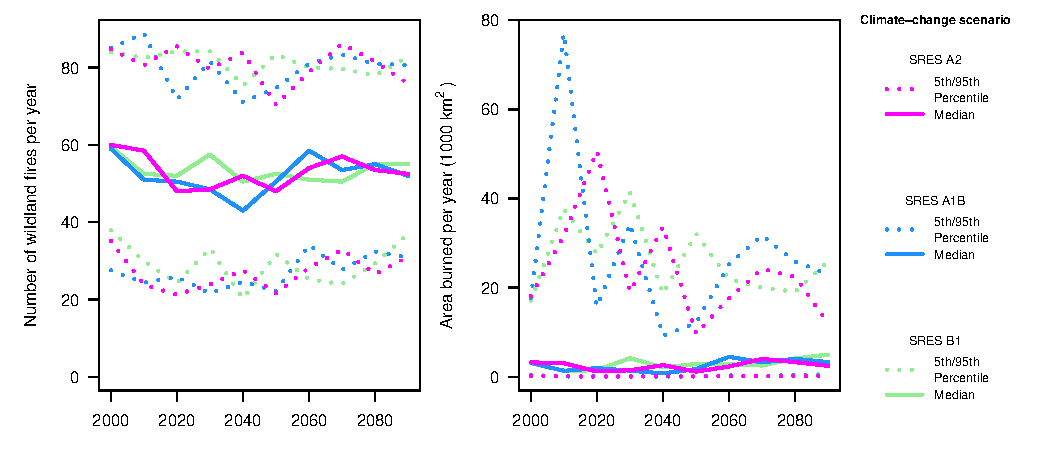
\includegraphics[width=\maxwidth]{figure/fire_change_ts_AK-1} \caption[Alaska]{Alaska}\label{fig:fire_change_ts_AK}
\end{figure}



All five following separate LCC graphs relate to figure 8.3 in the original document.
This uses strictly ALFRESCO output.

\subsection{Arctic}
\begin{figure}[H]
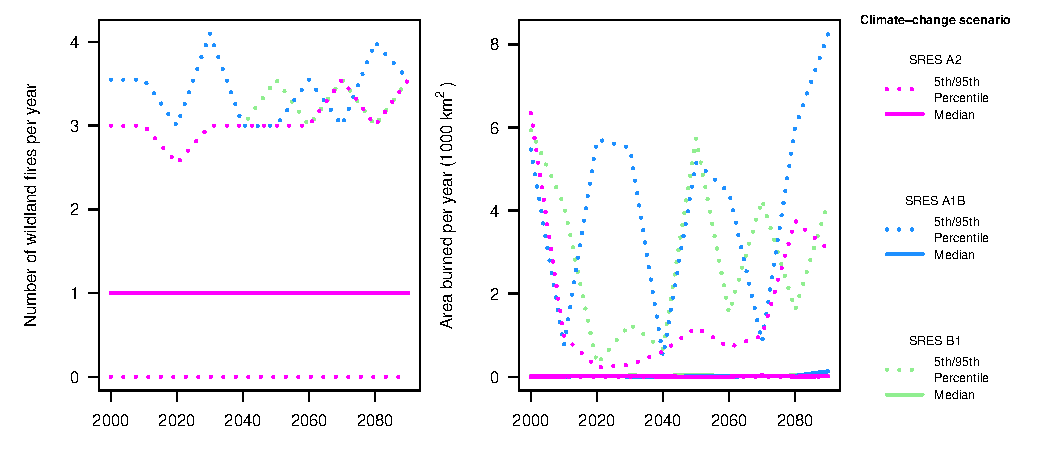
\includegraphics[width=\maxwidth]{figure/fire_change_ts_LCC1-1} \caption[Arctic]{Arctic}\label{fig:fire_change_ts_LCC1}
\end{figure}



\subsection{North Pacific}
\begin{figure}[H]
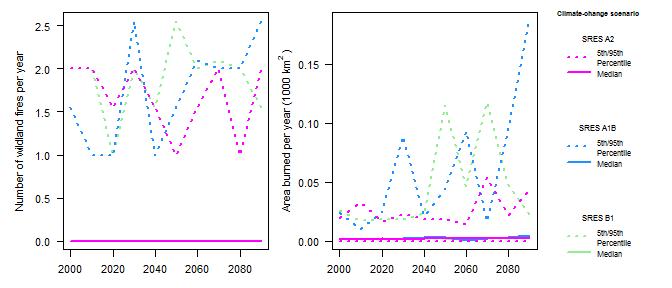
\includegraphics[width=\maxwidth]{figure/fire_change_ts_LCC2-1} \caption[North Pacific]{North Pacific}\label{fig:fire_change_ts_LCC2}
\end{figure}



\subsection{Northwest Interior Forest North}
\begin{figure}[H]
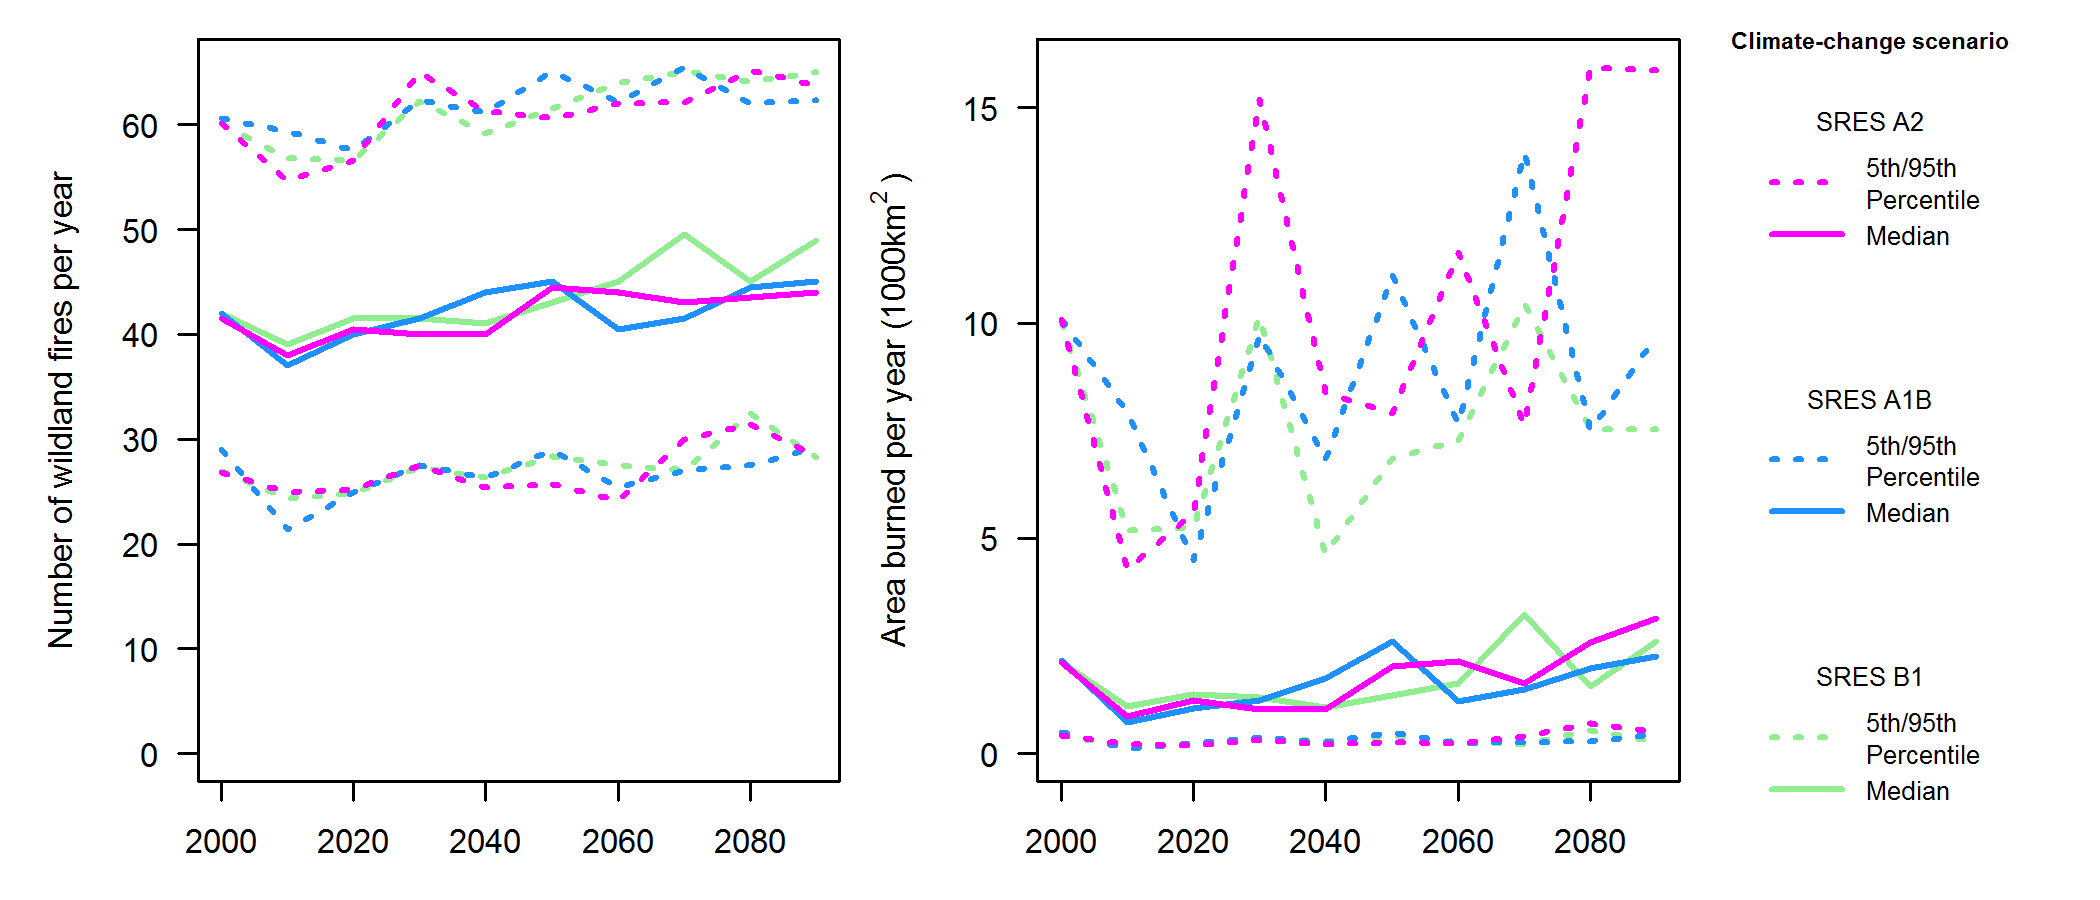
\includegraphics[width=\maxwidth]{figure/fire_change_ts_LCC3-1} \caption[Northwest Interior Forest North]{Northwest Interior Forest North}\label{fig:fire_change_ts_LCC3}
\end{figure}



\subsection{Northwest Interior Forest South}
\begin{figure}[H]
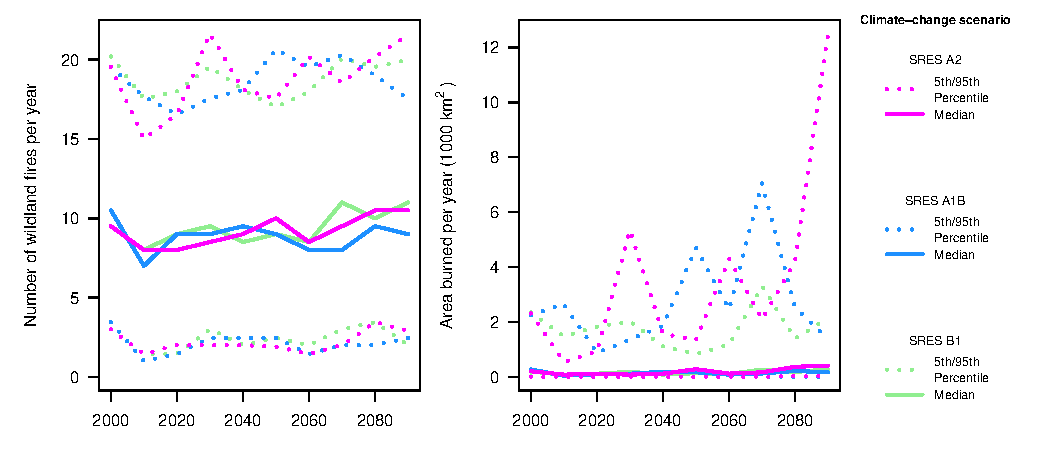
\includegraphics[width=\maxwidth]{figure/fire_change_ts_LCC4-1} \caption[Northwest Interior Forest South]{Northwest Interior Forest South}\label{fig:fire_change_ts_LCC4}
\end{figure}



\subsection{Western Alaska}
\begin{figure}[H]
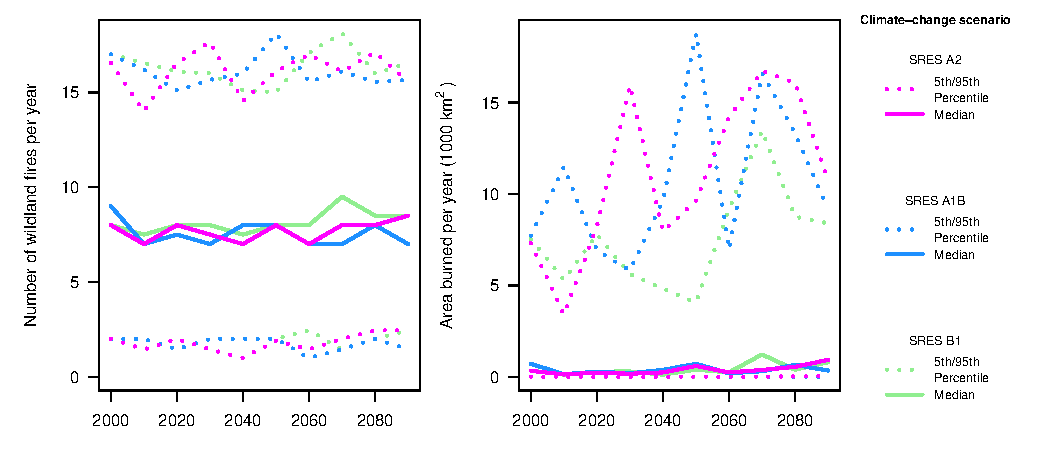
\includegraphics[width=\maxwidth]{figure/fire_change_ts_LCC5-1} \caption[Western Alaska]{Western Alaska}\label{fig:fire_change_ts_LCC5}
\end{figure}



\end{document}
